\subsection*{5.5 EXPERIMENT C: Scalability \& Stabilization}
\noindent The objective of the third experiment was to evaluate the scalability and stability of the I.C.U.M cooperative localization system as the network size increases. We aimed to determine how node density impacts the convergence speed and tracking accuracy, specifically testing whether larger clusters can maintain a stable coordinate frame in dynamic environments where a significant portion of the agents are moving.

\subsubsection*{Methodology}
\noindent Scalability was assessed using the same \textbf{On-Device RMSE} methodology described in Experiment A (Section 5.3), verifying the convergence behavior of the distributed spring-relaxation algorithm. By measuring the error of the firmware's internal state via the simulator's Oracle view, we directly evaluate the ability of large-scale meshes to self-organize through purely local interactions.\\

\noindent We conducted the experiment with varying node counts $[5, 10, 20, 35, 50, 75, 100]$. Two scenarios were executed for each configuration:
\begin{enumerate}
    \item \textbf{Static:} All nodes remain stationary to establish a baseline for optimal convergence.
    \item \textbf{Dynamic:} 70\% of the nodes follow the intermittent motion profile described in Section 5.2. This creates substantial topology turnover to test the system's re-convergence capabilities.
\end{enumerate}
The primary metric is the RMSE. Each configuration is run with multiple seeds to ensure statistical significance.The results demonstrate a clear relationship between node density and system stability. As shown in Figure \ref{fig:C_convergence_static}, in a static environment, all node configurations converge gradually over the 600-second duration, except for the 5-node cluster (RMSE $< 0.2$m at $t=20$s) and the 10-node cluster (RMSE $\approx 0.3-0.8$m at $t=120$s). For larger clusters $N \ge 20$, the relaxation process is computationally intensive. At $t=300$s, the system is still settling (RMSE ranges from $1.2$m for $N=75$ to $>2.3$m for $N=20$), only resolving to its minimum error floor by $t=600$s. Final convergence values are inversely proportional to density: $N=100$ achieves the highest precision ($\approx 0.09$m), followed by $N=75$ ($0.18$m) and $N=50$ ($0.36$m), while the sparser $N=35$ and $N=20$ configurations settle at a higher baseline ($0.69-0.77$m). 

To suppress UWB measurement noise, the distributed positioning algorithm uses a conservative learning rate $\alpha=0.2$. Consequently, position corrections must spread step-by-step across the network width. This acts as a slowing factor, where the "stiffness" of the overall map resolves slowly. For a network of diameter $D$, complete stabilization effectively requires $O(D^2)$ iterations, which explains the prolonged 600-second settling time required for the errors to diffuse out of the larger networks.

\begin{figure}[h]
\centering
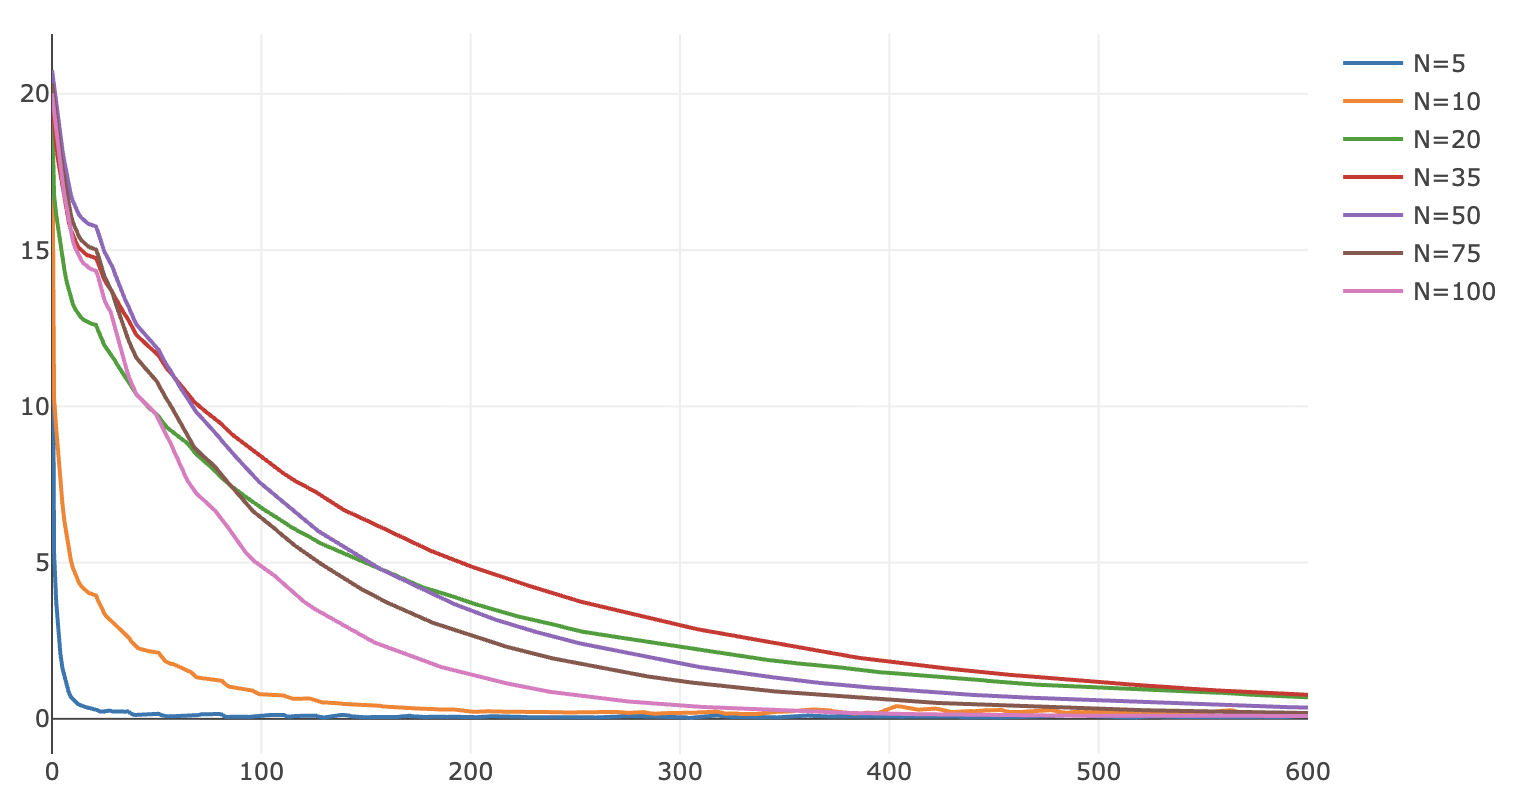
\includegraphics[width= 1\linewidth]{images'nshi/exp_c/c_static.png}
\caption{Graph depicting the Aligned RMSE ($y$-$axis$) over time ($x$-$axis$) with different amounts of nodes [5(blue), 10(orange), 20(green) 35(red) and 50(purple), 75(brown), 100(pink)]. In a static environment where nodes are not moving 
\label{fig:C_convergence_static}}
\end{figure}
\noindent In the dynamic scenario depicted in figure \ref{fig:C_convergence_moving}, the benefits of scale are more pronounced. With fewer nodes, the system is proportionally more susceptible to motion-induced errors and variance. Notably, intermediate node counts of 20 and 35 exhibit the highest instability, with 35 nodes reaching RMSE values as high as $1.45m$. This outlier performance is explained by the \textit{Rigidity Transition}—a phase change in random networks where the system shifts from being flexible to rigid. Below this threshold (e.g., $N=35$), the graph may be connected but remains "floppy," lacking the redundant triangular connections needed to uniquely define every node's position relative to the global map. When 70\% of the nodes move, the graph undergoes severe distortion that the cooperative positioning algorithm cannot correct quickly enough. In contrast, at $N \ge 50$, the network crosses the rigidity threshold, forming a stiff mesh that mechanically resists deformation, keeping RMSE consistently low, at around $0.13 - 0.37$m, despite the high dynamism.
\begin{figure}[h]
\centering
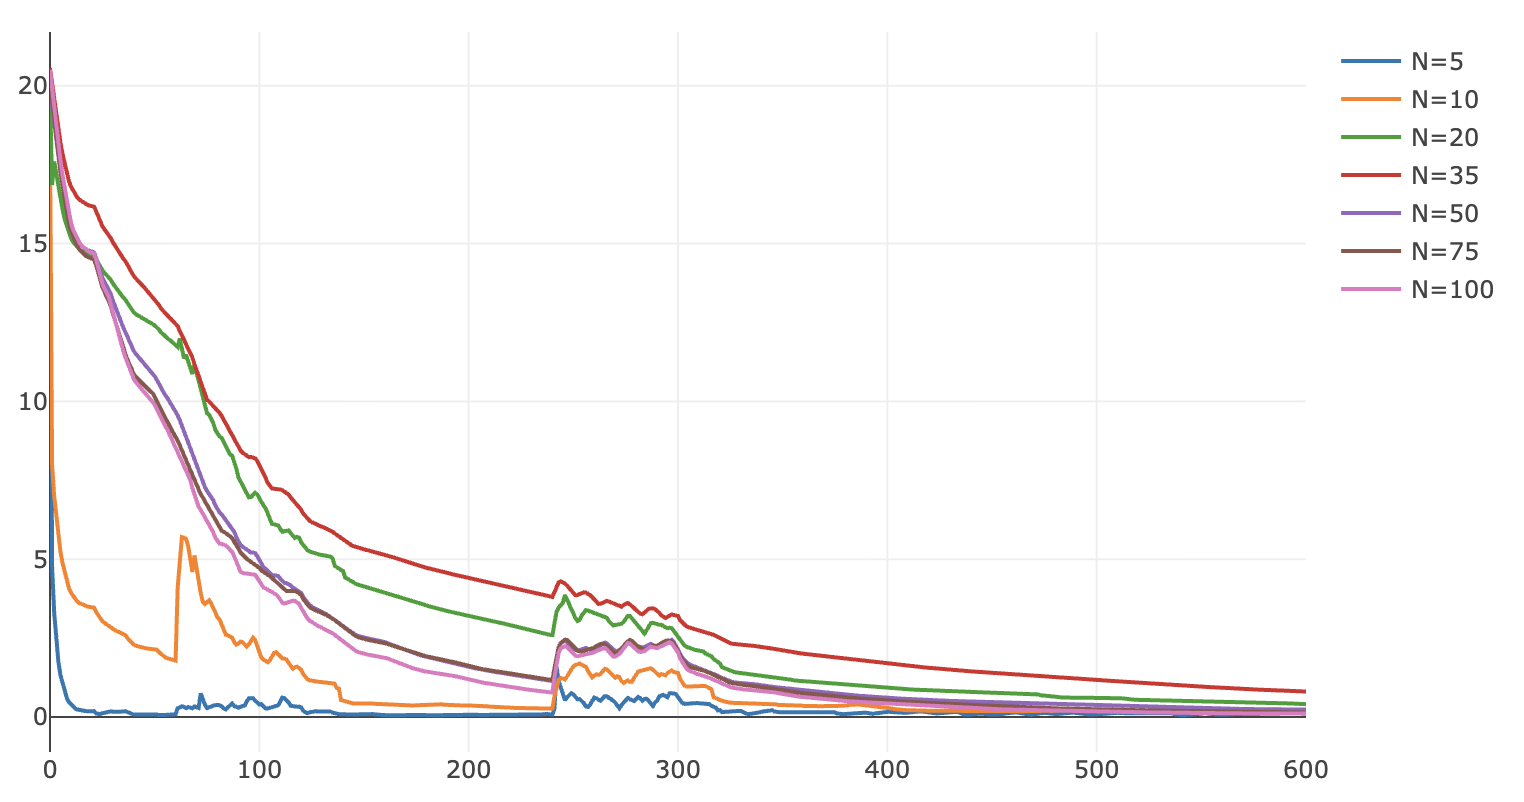
\includegraphics[width= 1\linewidth]{images'nshi/exp_c/c_50_pct_moving.png}
\caption{Graph depicting the Aligned RMSE ($y$-$axis$) over time ($x$-$axis$) with different amounts of nodes [5(blue), 10(orange), 20(green) 35(red) and 50(purple), 75(brown), 100(pink)]. 70 percent of the nodes moving, shows that 50 nodes increase in stabilization
\label{fig:C_convergence_moving}}
\end{figure}\\
Moreover, the data shows that 50 nodes increase in stabilization significantly. Specifically, configurations with 50 or more nodes maintain a consistently low RMSE, even with 70\% of the nodes in motion. At $t=600$s, $N=50$ resolves to $\approx 0.23$m, improving further with $N=75$ ($\approx 0.14$m) and $N=100$ ($\approx 0.11$m). 
This confirms that the cooperative algorithm effectively leverages the redundancy of larger swarms to reject outliers. Furthermore, movement actually \textit{aids} convergence in high-density scenarios ($N \ge 50$) through two mechanisms:
\begin{enumerate}
  \item \textbf{Topology Reshuffling:} The motion windows allow the network to change its shape. Nodes that were trapped in bad positions (like straight lines) are moved to new spots, helping the system find a better shape when they stop.
    \item \textbf{Motion-Assisted Correction:} The movement helps shake the system out of errors. Unlike a static network that can freeze in a wrong state, the "start-stop" pattern helps the algorithm settle into a more accurate configuration after each move.
    \item \textbf{Burst Sampling:} The ETM protocol triggers a $10\times$ increase in ranging frequency (from $0.1$ Hz to $1.0$ Hz) specifically \textit{during} the motion windows. This burst of high-density measurements allows the network to rapidly converge to the new toplogy before returning to a low-power maintenance state.
\end{enumerate}

\noindent However, this accuracy comes at the cost of communication bandwidth. Analysis of the messaging rate reveals that the average transmission frequency per node increases linearly with node density (from $\approx 30$ tx/node/min for 5 nodes to $\approx 800$ tx/node/min for 100 nodes). This load is driven by two distinct traffic classes:
\begin{itemize}
    \item \textbf{Heartbeat Messages ($O(N)$):} Periodic `HELLO` beacons reports are broadcast by every node. This traffic scales linearly with network size and provides the basic connectivity graph.
    \item \textbf{Ranging Exchanges ($O(N^2)$):} The active ranging process triggers the majority of the load. A single `RANGING\_POLL` broadcast elicits unicast `RANGING\_RESP` packets from all hearing neighbors. As density increases, the number of neighbors per node grows, causing a quadratic explosion in response traffic that saturates the channel.
\end{itemize}
Consequently, while the system is highly robust at scale, the total network load follows an $O(N^2)$ trend, which imposes a practical upper limit on size given the finite capacity of the wireless channel.
